%%%%%%%%%%%%%%%%%%%%%%%%%%%%%%%%%%%%%%%%%%%%%%%%%%%%%%%%%%%%%%%%%%%%%%%%%%%%%%%%
%2345678901234567890123456789012345678901234567890123456789012345678901234567890
%        1         2         3         4         5         6         7         8

\documentclass[letterpaper, 10 pt, conference]{ieeeconf}  % Comment this line out if you need a4paper
\usepackage{amsmath}
\usepackage{booktabs}
\usepackage{multirow}
\usepackage{graphicx}
%\usepackage{caption}
\usepackage{subcaption}
\usepackage[hidelinks]{hyperref}

%\documentclass[a4paper, 10pt, conference]{ieeeconf}      % Use this line for a4 paper

\IEEEoverridecommandlockouts                              % This command is only needed if 
                                                          % you want to use the \thanks command

\overrideIEEEmargins                                      % Needed to meet printer requirements.

% See the \addtolength command later in the file to balance the column lengths
% on the last page of the document

% The following packages can be found on http:\\www.ctan.org
%\usepackage{graphics} % for pdf, bitmapped graphics files
%\usepackage{epsfig} % for postscript graphics files
%\usepackage{mathptmx} % assumes new font selection scheme installed
%\usepackage{times} % assumes new font selection scheme installed
%\usepackage{amsmath} % assumes amsmath package installed
%\usepackage{amssymb}  % assumes amsmath package installed

\title{\LARGE \bf
Pose Estimation using ICP
}


\author{Nischal K N - nischal@seas.upenn.edu% <-this % stops a space
}


\begin{document}



\maketitle
\thispagestyle{empty}
\pagestyle{empty}


%%%%%%%%%%%%%%%%%%%%%%%%%%%%%%%%%%%%%%%%%%%%%%%%%%%%%%%%%%%%%%%%%%%%%%%%%%%%%%%%
\begin{abstract}

This project aims at determining the pose of an object using the 3D point cloud obtained from a depth camera. The pose is determined with respect to a 3D model of the object using iterative closest point(ICP). Two techniques are tried and compared here. Point to Point ICP and Point to Plane ICP are evaluated and the results obtained from both the methods are tabulated.

\end{abstract}


%%%%%%%%%%%%%%%%%%%%%%%%%%%%%%%%%%%%%%%%%%%%%%%%%%%%%%%%%%%%%%%%%%%%%%%%%%%%%%%%
\section{INTRODUCTION}
Interative closest point is an algorithm to register the difference between two point clouds. Here in this project it is used to determine the pose of a object with respect to its 3D model. The 3D model is used as a frame of reference. From this it is possible to determine the pose of the camera and trace the movement of camera wrt to the model. The performance of two ICP algorithm, namely point to point and point to plane is evaluated and the results are presented in Section \ref{sec:exp}. The dataset used is explained in Section \ref{sec:dataset}. First the object of interest is extracted from the point cloud using RANSAC and some filtering as explained in Section \ref{sec:gr}. The implementation of the two ICP are presented in Section \ref{sec:p2p} and \ref{sec:p2pl}.

\section{DATASET}
\label{sec:dataset}
The dataset used for the project consists of depth and RGB images of 2 objects, a drill and an liquid container. It consists of a series of 447 depth and RGB images as the camera moves around the object of interest. Also a 3D model of the objects are used as the reference frame shown in Fig. \ref{fig:model}. The vicon data provided for the camera pose is not used. Fig \ref{fig:data} shows a sample RGB image and the corresponding point cloud.

\begin{figure}
\begin{subfigure}[b]{0.5\textwidth}
	\centering
   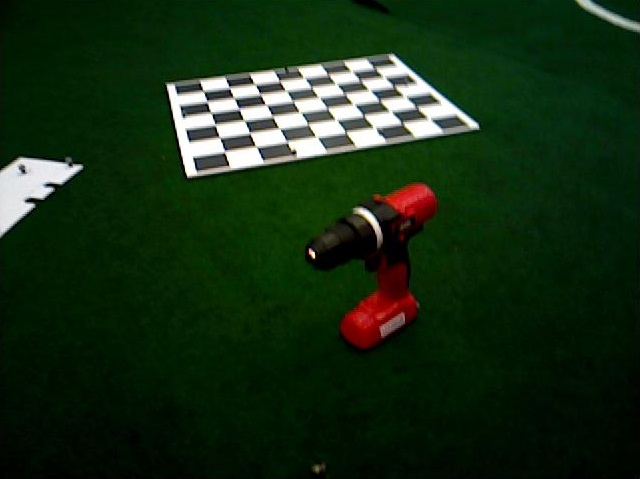
\includegraphics[scale = 0.35]{rgb.jpg}
   \caption{RGB image}
   \label{fig:init} 
\end{subfigure}

\begin{subfigure}[b]{0.5\textwidth}
	\centering
   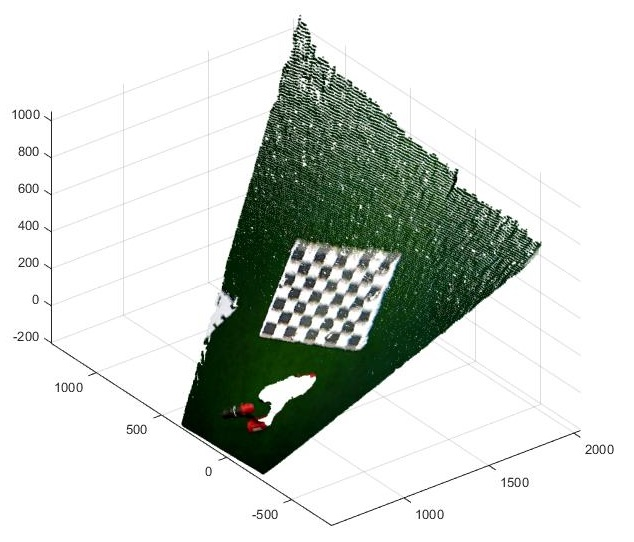
\includegraphics[scale =0.35]{depth.jpg}
   \caption{Point cloud of corresponding depth image}
   \label{fig:mean}
\end{subfigure}

\begin{subfigure}[b]{0.5\textwidth}
	\centering
   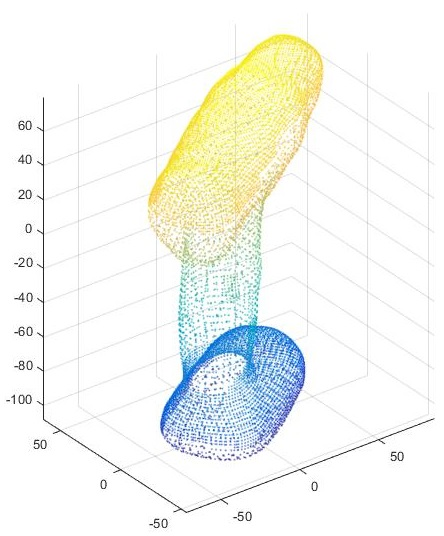
\includegraphics[scale =0.35]{model.jpg}
   \caption{Point cloud of 3D model}
   \label{fig:model}
\end{subfigure}
\caption{Pose initialization by removing translation}
\label{fig:data}
\end{figure}

\section{Ground Removal and filtering}
\label{sec:gr}
The first step is to extract the object from the 3D point cloud. This is performed in three steps. First a threshold is set on the maximum depth of the point cloud since the object is present close to the camera. Then RANSAC is applied to detect the ground plane with a very small threshold of 15mm and for 100 iterations. This removes most of the ground plane but leaves behind some residue that are removed with filtering. The output after RANSAC is shown in Fig. \ref{fig:ransac} with removed ground plane in red and object points in green. To remove this residue, the median of the point cloud is calculated and any points within 120mm of the median are retained. This value is choosen because the object has an approximate dimension of $160\times120\times200mm$. Any points that are further than 120mm is removed. The output is shown in Fig. \ref{fig:clean}.

\begin{figure*}
\centering
\begin{subfigure}{.3\textwidth}
  \centering
  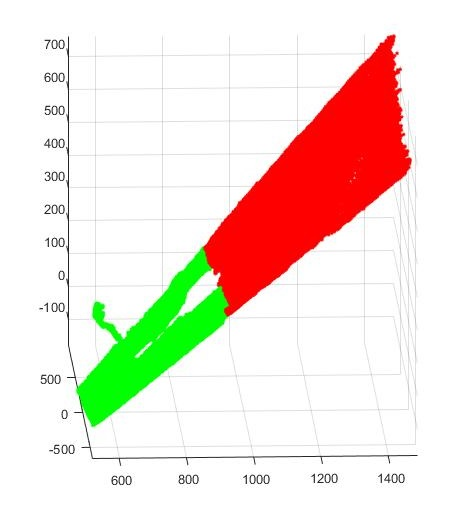
\includegraphics[scale=0.3]{thresholding.jpg}
  \caption{Thresholding the depth}
  \label{fig:thresh}
\end{subfigure}%
\begin{subfigure}{.3\textwidth}
  \centering
  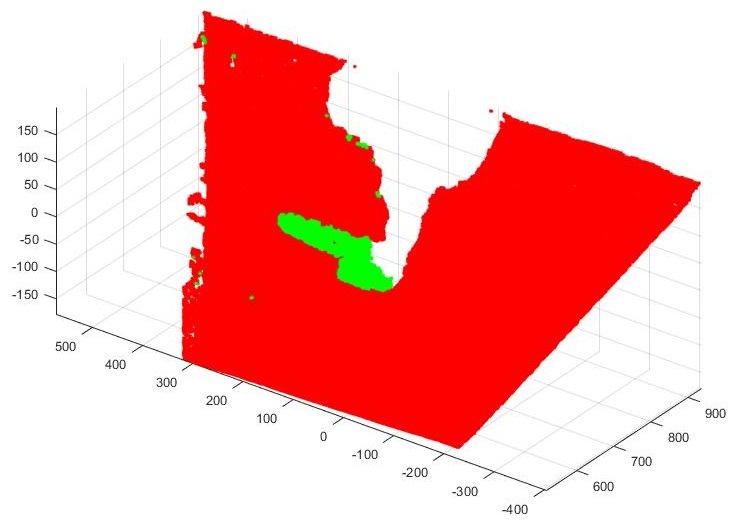
\includegraphics[scale=0.3]{ransac2.jpg}
  \caption{RANSAC with noise}
  \label{fig:ransac}
\end{subfigure}
\begin{subfigure}{.3\textwidth}
  \centering
  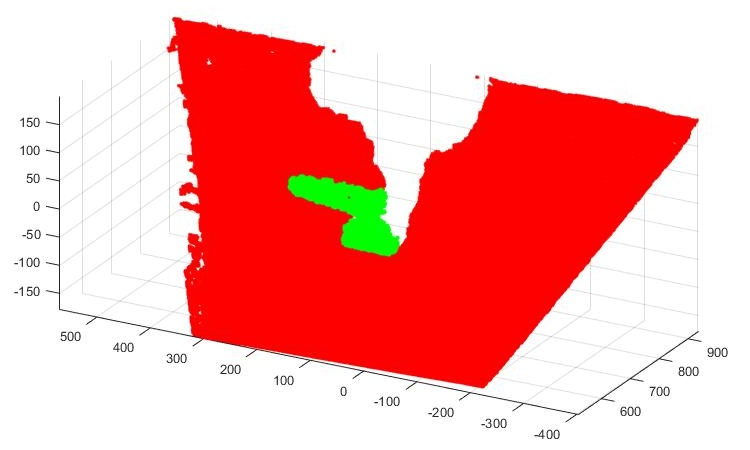
\includegraphics[scale=0.3]{clean.jpg}
  \caption{Afetr filtering based on distance from median}
  \label{fig:clean}
\end{subfigure}%
\caption{Ground removal process. Green Pixels are retained and Red pixels eliminated at each step}
\label{fig:gr}
\end{figure*}


\section{Point to Point ICP}
\label{sec:p2p}
This technique follow the procedure described in \cite{c1}. It uses SVD to determine the rotation matrix. The algorithm is as follows
\begin{enumerate}
\item Determine the corresponding points of the model to each point of our point cloud using knnsearch.
\item Determine $p$ and $p'$ given as
\begin{align*}
p =&\; \frac{1}{N}\sum_{i=1}^N p_i \\
p' =&\; \frac{1}{N}\sum_{i=1}^N p_i' \\
\end{align*}
where $p_i$ and $p_i'$ are the points in the model and depth point clouds.
\item Determine $q$ and $q'$ using
\begin{align*}
q_i =&\; p_i - p \\
q_i' =&\; p_i' - p' \\
\end{align*}
\item Calculate the 3x3 matrix H and find its SVD
\begin{align*}
H =&\; \sum_{i=1}^N q_iq_i'^{t} \\
H =&\; U \Lambda V^t
\end{align*}
\item Finally calculate the Rotation and translation matrix using
\begin{align*}
R =&\; VU^t \\
P =&\; p' - Rp
\end{align*}
\end{enumerate}
This procedure is repeated iteratively by using the determined R and T to initial the pose of the point cloud for the next iteration until the value of R and T stabilizes.

\section{Point to Plane ICP}
\label{sec:p2pl}
Another version of ICP tested was point to plane\cite{c2}. Here the surface normals of the models are computed which are then compared with the point cloud to determine R and T.
\begin{enumerate}
\item Calculate the normals for all points of the model point cloud.
\item Do a KNN correspondence search to determine the closest model normals for the object point cloud.
\item Calculate the b matrix and A matrix as follows
\begin{align*}
b =&\;
\begin{bmatrix}
n_{1x}d_{1x} + n_{1y}d_{1y} + n_{1z}d_{1z} ... \\
... - n_{1x}s_{1x} - n_{1y}d_{1y} - n_{1z}d_{1z} \\
n_{2x}d_{2x} + n_{2y}d_{2y} + n_{2z}d_{2z} ... \\
... - n_{2x}s_{2x} - n_{2y}d_{2y} - n_{2z}d_{2z} \\
\vdots \\
n_{Nx}d_{Nx} + n_{Ny}d_{Ny} + n_{Nz}d_{Nz} ... \\
... - n_{Nx}s_{Nx} - n_{Ny}d_{Ny} - n_{Nz}d_{Nz} \\
\end{bmatrix} \\
\intertext{Where d is the points in model point cloud, s are the points in the object point cloud anf n are the normals}
A = &\;
\begin{bmatrix}
a_{11} & a_{12} & a_{13} & n_{1x} & n_{1y} & n_{1z} \\
a_{21} & a_{22} & a_{23} & n_{2x} & n_{2y} & n_{2z} \\
\vdots & \vdots & \vdots & \vdots & \vdots & \vdots \\
a_{N1} & a_{N2} & a_{N3} & n_{Nx} & n_{Ny} & n_{Nz} \\
\end{bmatrix}
\intertext{where }
a_{i1} =&\; n_{iz}s_{iy} - n_{iy}s_{iz} \\
a_{i2} =&\; n_{ix}s_{iz} - n_{iz}s_{ix} \\
a_{i3} =&\; n_{iy}s_{ix} - n_{ix}s_{iy} \\
\end{align*}
\item x consisting of R and T is calculated using
\begin{align*}
x =&\; A^{-1}b
\intertext{where}
x =&\;
\begin{bmatrix}
\alpha & \beta & \gamma & t_x & t_y & t_z \\
\end{bmatrix}
\end{align*}
The R and T matrix are obtained from x
\end{enumerate}
This procedure is repeated iteratively by using the determined R and T to initial the pose of the point cloud for the next iteration until the value of R and T stabilizes.

\begin{figure}
\centering
   \begin{subfigure}[b]{0.5\textwidth}
   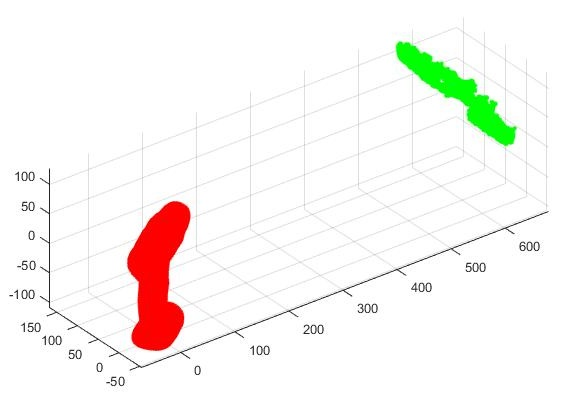
\includegraphics[scale = 0.5]{init2.jpg}
   \caption{Initial pose with large translation}
   \label{fig:init} 
\end{subfigure}

\begin{subfigure}[b]{0.5\textwidth}
   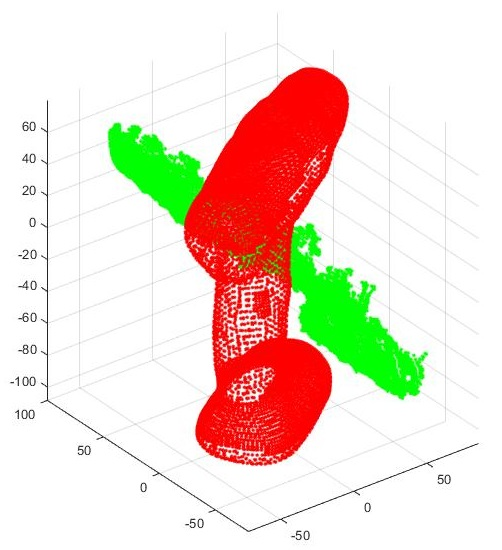
\includegraphics[scale =0.5]{mean.jpg}
   \caption{Large pose corrected by mean centering}
   \label{fig:mean}
\end{subfigure}
\caption{Pose initialization by removing translation}
\end{figure}

\section{Initialization of ICP pose}
\label{sec:init}
ICP algorithm is a local algorithm. Hence an approximate initial pose must be defined so that it converges well. In order to remove the large translation, the object is mean centered. This change is shown in Fig. \ref{fig:mean}. Then two approaches were experimented to define the initial pose, coarse search and initializing with pose of previous frame.
\subsection*{Coarse Search}
The initial pose of the object was defined to be from a set of pitch and yaw angles 0 to 180 at increments of 30 degree. For each of the combinations of pitch and yaw, ICP was run for 50 iterations and the error was recorded. The error was measured as the sum of distance between the correspondence points obtained by knn search. The pair of pitch and yaw angles that had the minimum error was chosen as the initial pose for the ICP for that frame. However this method was too slow due to the number of iteration of ICP every frame had to go through.
\subsection*{Initializing with pose of previous frame}
This method was used to overcome the slow speed of coarse search. Instead of searching through the entire space of pitch and yaw angles, the pose obtained from the previous frame was used as the initial pose for the current frame and then the incremental pose change was computed. This made is sufficiently quicker. The initial pose was set manually

\section{Experiments and Results}
\label{sec:exp}
For both the datasets, both the above mentioned ICP was run by initializing the pose with the pose of the previous frame. The results of some of the frames are tabulated in Table \ref{tab:drill} and \ref{tab:liquid}. The number of iterations required to converge and the time taken are also specified. It is seen that point to plane ICP performs much faster than point to point ICP and also was more robust in converging. Additionally a link to GIF image of the process of convergence for each of these are provided.

\begin{table*}
\centering
\caption{Comparison of point to point and point to plane ICP for drill}
\label{tab:drill}
\begin{tabular}{ccccccc}
Frame Number & \multicolumn{3}{c}{Point to Pplane ICP} & \multicolumn{3}{c}{Point to Point ICP} \\ 
\toprule
1 & \multicolumn{3}{c}{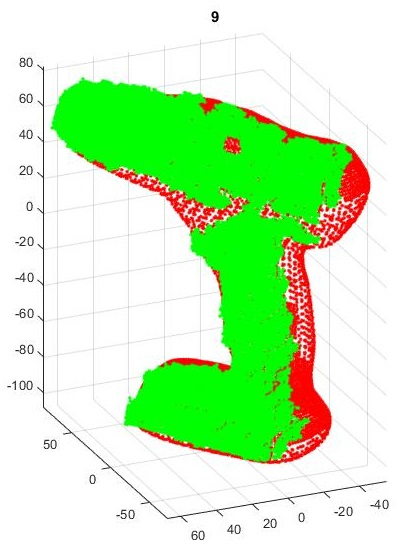
\includegraphics[scale=0.43]{d1p.jpg}} & \multicolumn{3}{c}{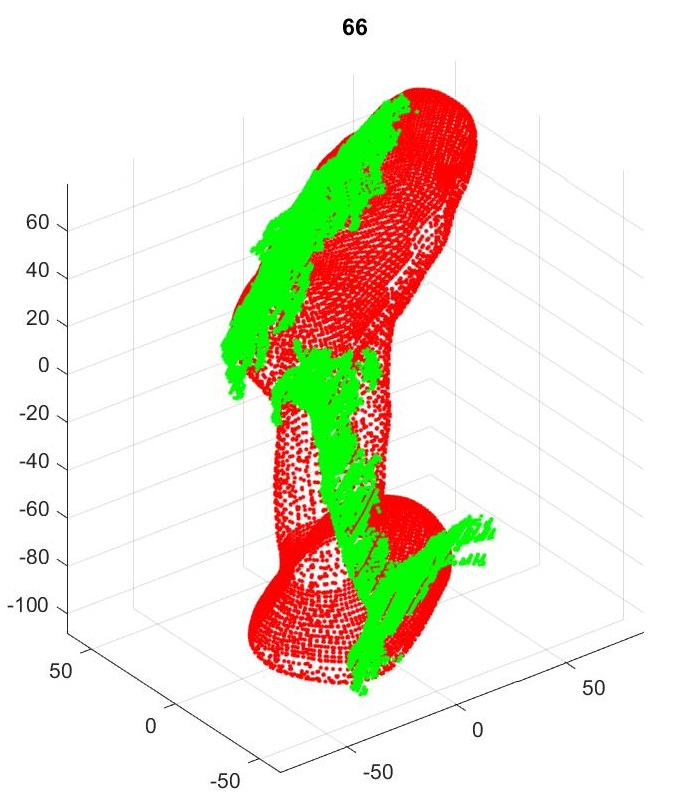
\includegraphics[scale=0.3]{d1o.jpg}}\\ 
 & Time: 2.12s & Iterations: 9 & \href{http://gph.is/1WElekI}{\textbf{GIF(click)}} & Time: 11.18s & Iterations: 66 & \href{http://gph.is/1rPINfj}{\textbf{GIF(click)}}\\ 
\midrule
200 & \multicolumn{3}{c}{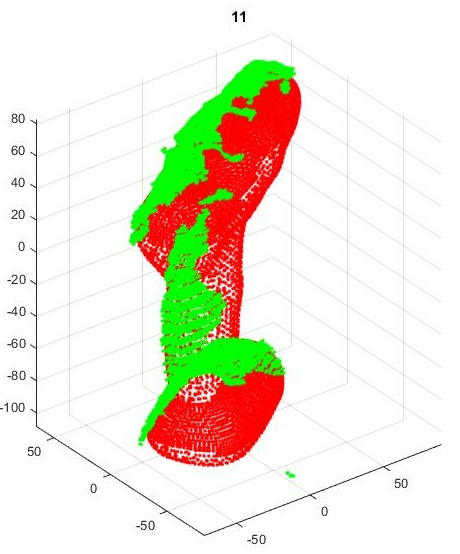
\includegraphics[scale=0.43]{d200p.jpg}} & \multicolumn{3}{c}{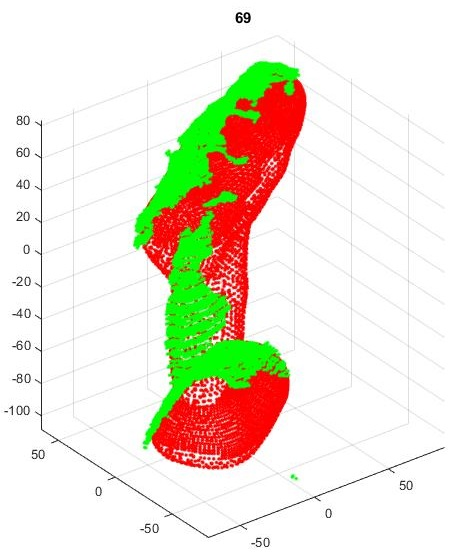
\includegraphics[scale=0.43]{d200o.jpg}}\\ 
 & Time: 2.30s & Iterations: 11 &  & Time: 10.92s & Iterations: 69 & \\ 
\midrule
400 & \multicolumn{3}{c}{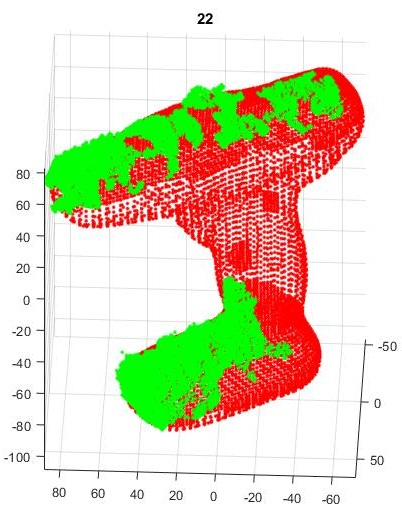
\includegraphics[scale=0.43]{d400p.jpg}} & \multicolumn{3}{c}{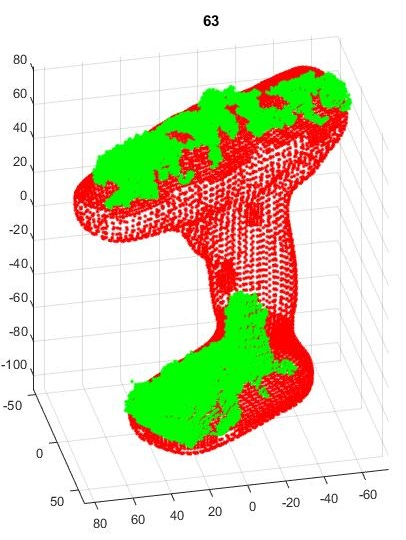
\includegraphics[scale=0.43]{d400o.jpg}}\\ 
 & Time: 3.60s& Iterations: 22 &  & Time: 9.57s& Iterations: 63& \\ 
\bottomrule
\end{tabular} 
\end{table*}

\begin{table*}
\centering
\caption{Comparison of point to point and point to plane ICP for liquid container}
\label{tab:liquid}
\begin{tabular}{ccccccc}
Frame Number & \multicolumn{3}{c}{Point to Point ICP} & \multicolumn{3}{c}{Point to Plane ICP} \\ 
\toprule
10 & \multicolumn{3}{c}{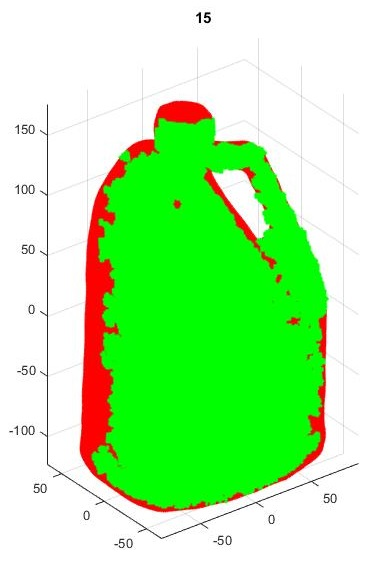
\includegraphics[scale=0.43]{l10p.jpg}} & \multicolumn{3}{c}{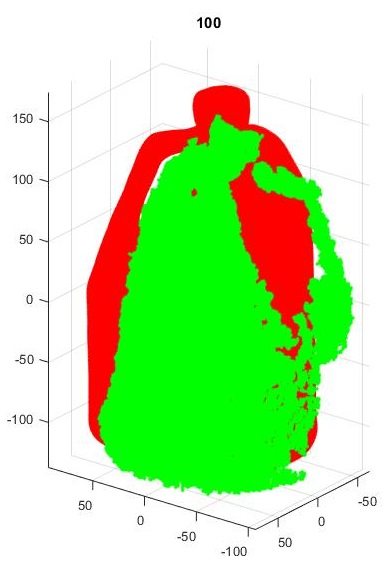
\includegraphics[scale=0.43]{l10o.jpg}}\\ 
 & Time: 6.42s& Iterations: 15& \href{http://gph.is/1rg24Wp}{\textbf{GIF(click)}} & Time: 44.72s & Iterations: 100 (Did not converge)& \href{http://gph.is/1rPJGo2}{\textbf{GIF(click)}}\\ 
\midrule
210 & \multicolumn{3}{c}{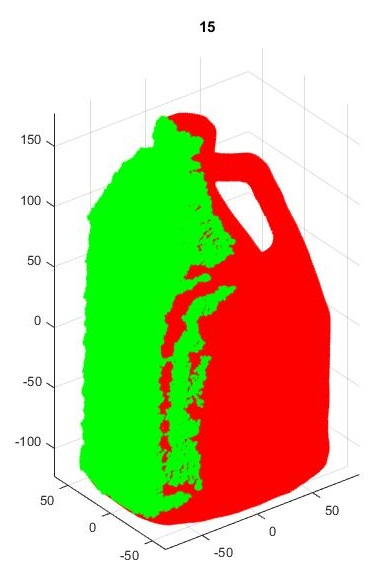
\includegraphics[scale=0.43]{l210p.jpg}} & \multicolumn{3}{c}{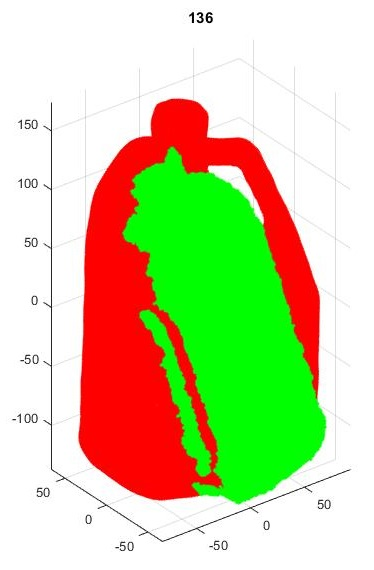
\includegraphics[scale=0.43]{l210o.jpg}}\\ 
 & Time: 6.80s & Iterations: 15 & & Time: 74.50s& Iterations: 136& \\ 
\midrule
410 & \multicolumn{3}{c}{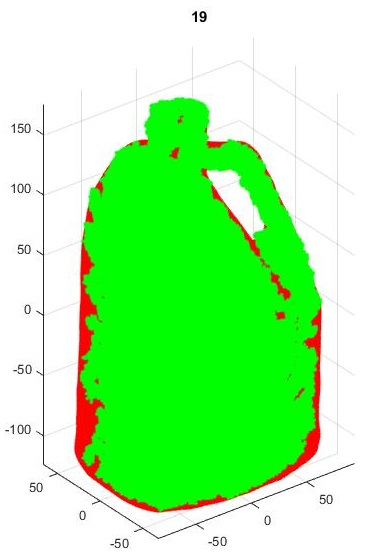
\includegraphics[scale=0.43]{l410p.jpg}} & \multicolumn{3}{c}{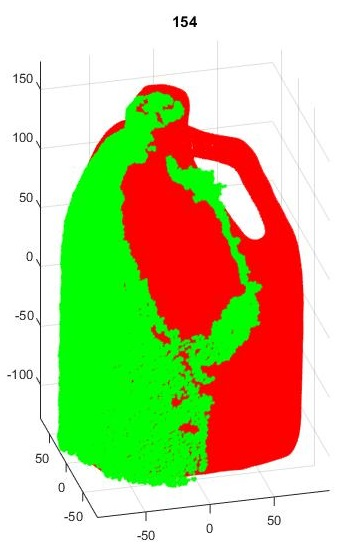
\includegraphics[scale=0.43]{l410o.jpg}}\\ 
 & Time: 7.84s& Iterations: 19& & Time: 62.49s & Iterations: 154 & \\ 
\bottomrule
\end{tabular} 
\end{table*}

\section{Future Work}
\begin{itemize}
\item The R and T values calculated for each frame can be used to find the camera pose/camera motion around the object.
\item Go ICP can be used to find the global minima.
\end{itemize}

\begin{thebibliography}{99}

\bibitem{c1} Arun, K. Somani, Thomas S. Huang, and Steven D. Blostein. "Least-squares fitting of two 3-D point sets." Pattern Analysis and Machine Intelligence, IEEE Transactions on 5 (1987): 698-700.

\bibitem{c2}Low, Kok-Lim. "Linear least-squares optimization for point-to-plane icp surface registration." Chapel Hill, University of North Carolina 4 (2004).


\end{thebibliography}




\end{document}
